\section{流形}
	\textbf{微分流形}$M$是一个集合,$n$维流形是指该集合局部同胚与$\mathbb{R}^n$上的开集,所谓同胚是可逆的光滑映射;\\

	\textbf{微分流形}是在拓扑流形基础上施加了进一步约束,称为\textbf{微分结构},具体来说,\\

	$p,q \in M$,$p$的邻域为$U$,$q$的邻域为$V$,则\\

	根据定义,存在同胚映射$\phi: U\mapsto \mathbb{R}^n$,$\psi: U\mapsto \mathbb{R}^n$,对$U\cap V$上的点,需符合映射,
	$$
		\phi\circ\psi^{-1}: \mathbb{R}^n \mapsto \mathbb{R}^n
	$$
	是光滑映射。\\

	根据定义,流形是有维数的,很明显$\mathbb{R}^n$均为$n$维流形,流形定义是脱离坐标系的。

\subsubsection*{微分同胚}

两个微分流形$M,M^\prime$,如果存在可逆的光滑映射$f: M\mapsto M^\prime$,且其逆映射$f^{-1}$也光滑,则称$M,M^\prime$ \textbf{微分同胚}。\\

两个群同构则认为其“完全一样”,相似的两个流形微分同胚则认为“完全一样”。

\subsubsection*{二维球面$S^2$}
三维空间中的球面是一个2维流形,用$S^2$表示,为什么是2维流形呢?在半径确定的情况下,用两个角度即可表示球面上任意点,所以是2维。\\

若要通过坐标系描述$S^2$,则需在三维空间中完成,因此,准确说,$S^2$是嵌入三维空间的二维流形。

\subsubsection*{矢量}
	在$R^n$中“矢量”的意义是明确的,是有大小、有方向的“箭头”,并且与箭头的起始位置无关。\\

	一般流形上没有定义“大小”、“方向”这些概念,那矢量的本质是什么呢?\\

	考虑某个向量$\mathbf{v} = (v_1,v_2,v_3)$,函数$f(x,y,z)$沿$\mathbf{v}$的方向导数为,
	$$
		D_\mathbf{v}(f) \equiv\nabla_f \cdot \mathbf{v}
	$$

	由此看出矢量$\mathbf{v}$可看作$\mathscr{F} \mapsto \mathbb{R} $的映射,$\mathscr{F}$是$\mathbb{R}^3\mapsto \mathbb{R}$的函数集合。\\

	容易验证,$D_\mathbf{v}$是线性映射,

	$$
		D_\mathbf{v}(\alpha f+ \beta g) = \alpha D_\mathbf{v}(f) + \beta D_\mathbf{v}(g)
	$$

	且满足莱布尼兹律,
	$$
		D_\mathbf{v}(fg) = fD_\mathbf{v}(g) + gD_\mathbf{v}(f)
	$$

	由此可见,矢量本质是一个线性映射,推广到一般流形,定义为:\\

	\textbf{流形$M$上的矢量$v$是$\mathscr{F}_M \mapsto \mathbb{R} $的,满足莱布尼兹律的线性映射。}\\

	即,
	\begin{equation} \label{v_linear}
		v(\alpha f+ \beta g) = \alpha v(f) + \beta v(g),\forall f,g \in \mathscr{F}_M,\forall \alpha,\beta \in \mathbb{R}
	\end{equation}

	及
	\begin{equation} \label{v_leb}
		v(fg) = fv(g) + gv(f),\forall f,g \in \mathscr{F}_M
	\end{equation}

	大多数几何书上对矢量的定义就到此为止了,很难从这个定义“想象”出流形上的矢量到底长什么样子,因为这个定义没有揭示方向导数更本质意义。\\

	\begin{figure}[H]
		\begin{center}
			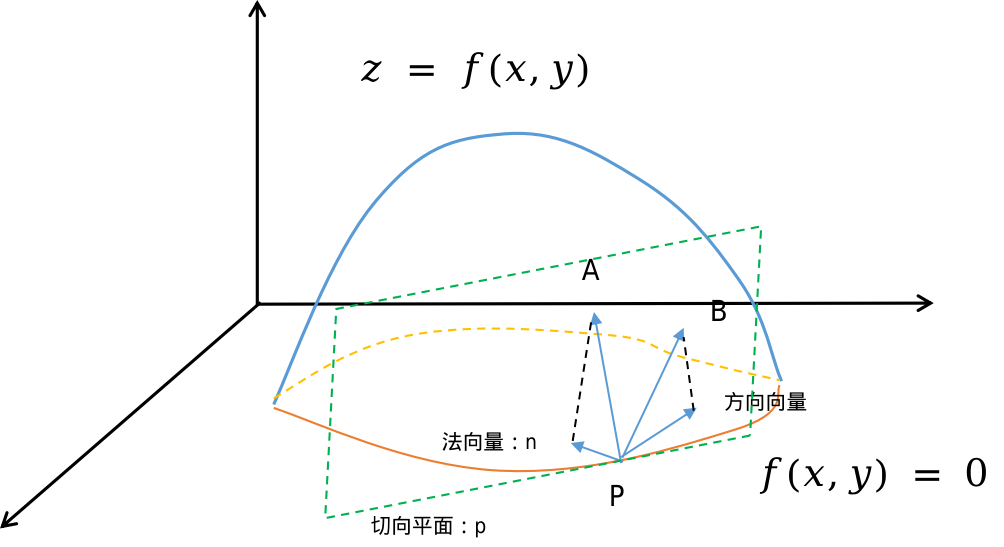
\includegraphics[width=0.8\textwidth]{images/direct_vector.png}
		\end{center}
		\caption{方向向量、方向导数、法向量、切平面}
	\end{figure}	

	如图所示,$z=f(x,y)$的曲面代表一座山,曲面在$P$的切面是绿色平面$p$,$P$点对应的等高面是$f(x,y) = 0$\\

	可以沿着$PA,PB$两个方向(称为\textbf{方向向量})走,因为必须顺着山坡走,所以$PA,PB$都相切于曲面,也就是说$PA,PB$都位于曲面在$P$点的切面中。\\

	这非常重要,这说明\textbf{曲面的方向向量是曲面切平面中的向量,即曲面的切向量。}\\

	$PA$在等高面的投影是曲线$f(x,y) = 0$的法向量$n$,也是$z=f(x,y)$的\textbf{梯度向量};而$PB$在等高面的投影是一个一般向量。\\

	沿着哪个方向爬会更快呢?这就是所谓方向导数的问题,方向导数反应的是沿着某个方向函数值的增量。\\

	注意到,$PA,PB$只有在法向量$n$上的投影才能带来$z$的增量,在垂直于法向量的方向,函数没有定义,增量为了$0$;\\

	各种书上会经常指着$PA,PB$的投影为方向向量,实际上$PA,PB$才是真正的方向向量,二者是一一对应的。\\

	如此可以明确,\\

	\textbf{曲面的方向向量就是切向量,按切向量可计算方向导数,即函数增量;反之,能计算方向导数的算子就是切向量。}\\

	所以,流形上的矢量推广要做到,

	\begin{itemize}
		\item 流形上的矢量是曲面上向量的推广,反映到二维曲面上,应是曲面的切向量。
		\item 一元函数的切空间是一条直线($\mathbb{R}^1$),二元函数的切空间是一个平面($\mathbb{R}^2$),$n$维流形的切空间应该是$\mathbb{R}^n$。
	\end{itemize}
	

	只要能根据流形上矢量的定义规则验证第二点,那第一点自然也就成立了,那接下来的任务是证明流形的切空间与$\mathbb{R}^n$同构。

\subsubsection*{切空间}

	流形$M$在$p$点的切空间记为$V_p$,根据定义是一些满足(\ref{v_linear},\ref{v_leb})的算子,需定义数乘和加法来构成线性空间,
	$$
		v(\alpha f) = \alpha v(f), \forall v \in V_p
	$$

	$$
		(v + \nu )f = v(f) +\nu(f), \forall v,\nu \in V_p 
	$$

	接下来需证明$\mathbb{R}^n$与$V_p$线性同构。\\

	首先构造一个从$\mathbb{R}^n$到$V_p$的映射,
	$$
		\mathbf{v} \mapsto D_v = \sum_{i=1}^nv^i\frac{\partial f}{\partial x^i}\Big|_p
	$$

\subsubsection*{曲线切矢}


\subsubsection*{单参微分同胚群}
定义映射,
$$
	\phi:\mathbb{R} \times M \mapsto M
$$

则
$$
	G \equiv \left\lbrace \phi_t: M\mapsto M|t \in \mathbb{R} \right\rbrace
$$

其中$\phi_t = \phi(t,\cdot)$为微分同胚,则$G$构成群,群乘法为复合映射,称为\textbf{单参微分同胚群}。\\

很明显,$G$与$\mathbb{R}$同构。


\subsubsection*{切空间}
回想一下,一元函数的切线是一维的,二元函数的切面是二维的,n元函数存在n个偏导数,其切空间是n维。\\

与此类似,$n$维流形$M$在$p$点的切空间为$V_p$,也是$n$维的\textbf{向量空间},$M$上每个点都存在一个$n$维切空间。\\

$V_p$中每个向量都是$p$点的切向量。

\subsubsection*{曲线}
流形$M$上的曲线,是一个映射,
$$
	\gamma(t): \mathbb{R} \mapsto M
$$

比如$S^2$上的点可表示为$(\alpha,\beta)$,表示赤道线的曲线为,
$$
	\gamma(t): [0,2\pi] \mapsto S^2
$$

$$
	\gamma(t) = (t,0), t\in [0,2\pi]
$$

\subsubsection*{度规}
可以在流形上赋予某种距离度量方式称为\textbf{度规},比如在$\mathbb{R}^n$中赋以欧式距离,在$S^2$中赋以球面距离。一旦有了度规,会导出内积、夹角、测地线等概念,赋以度规的流形称为\textbf{黎曼流形}或\textbf{黎曼空间}。

\subsubsection*{测地线}
粗略理解,测地线就是黎曼流形上两点间距离最短的那条线,比如欧式空间中的直线,$S^2$上的大圆弧。\\

结论:流形上的一个点及该点的切向量,可唯一确定一条测地线。\\

测地线也是曲线,也有对应的参数方程。

\subsubsection*{指数映射}
流形的维数与切空间的维数一致,那两个集合之间存在什么关系呢?\\

结论:在\textbf{黎曼流形}上,$T_pM$与$M$之间存在指数映射,
$$
	\exp:T_pM \mapsto M
$$

具体映射构造如下,
\begin{itemize}
\item 取点$p$及$T_pM$中的某个向量$A$,确定一条测地线$\gamma_A(t)$,$p$点的参数为$t_p$
\item 将$\gamma(t_p+1)$对应的点定义为映射的像,
\end{itemize}

$$
	\exp(p,A) = \gamma_A(t_p+1)
$$

通常取$p$点测参数值为$0$,则指数映射为,
$$
	\exp(p,A) = \gamma_A(1)
$$

如此,可将$T_pM$映射到$M$,当然任何一个点的切空间都可以映射到$M$,哪个点切空间更有代表性呢?\\

在流形上没有特殊点,需在李群上考虑这个问题。\\

要注意,虽然名字是指数映射,但这个映射跟“指数”操作没有任何关系。\\

\textit{注意,指数映射是定义在黎曼流形上,如果没有度规,就不是黎曼流形,就无法定义指数映射。}